\documentclass[11pt]{article}
 
\usepackage[top=0.75in, bottom=1.25in, left=1in, right=1in]{geometry} 
\usepackage{amsmath,amsthm,amssymb} %this is THE math package
\usepackage{mathtools}
\usepackage{tikz}
\usepackage{graphicx}
\usepackage{fancybox}
\usepackage{hyperref}
\usepackage{varwidth}
\usepackage{mdframed}
\usepackage{mathrsfs}
\usepackage[most]{tcolorbox}
%------------------------
%Fonts I use, uncomment if you like to use them.
%The first is the general font, and the second a math font
\usepackage{mathpazo}
\usepackage{eulervm}

%------------------------
%This is so that we have standard fonts for the double-stroked symbols
%for reals, naturals etc. regardless of what font you use.
%Don't comment
\AtBeginDocument{
  \DeclareSymbolFont{AMSb}{U}{msb}{m}{n}
  \DeclareSymbolFontAlphabet{\mathbb}{AMSb}}
%------------------------
\usepackage{graphicx}
\graphicspath{ {./images/} }
%----------------------------------------------
%User-defined environments
%Commented because we're not using them in this document
%The only uncommented ones are the Problem and Solution environment

% \newenvironment{theorem}[2][Theorem]{\begin{trivlist}
% \item[\hskip \labelsep {\bfseries #1}\hskip \labelsep {\bfseries #2.}]}{\end{trivlist}}
% \newenvironment{lemma}[2][Lemma]{\begin{trivlist}
% \item[\hskip \labelsep {\bfseries #1}\hskip \labelsep {\bfseries #2.}]}{\end{trivlist}}
% \newenvironment{exercise}[2][Exercise]{\begin{trivlist}
% \item[\hskip \labelsep {\bfseries #1}\hskip \labelsep {\bfseries #2.}]}{\end{trivlist}}
% \newenvironment{question}[2][Question]{\begin{trivlist}
% \item[\hskip \labelsep {\bfseries #1}\hskip \labelsep {\bfseries #2.}]}{\end{trivlist}}
% \newenvironment{corollary}[2][Corollary]{\begin{trivlist}
% \item[\hskip \labelsep {\bfseries #1}\hskip \labelsep {\bfseries #2.}]}{\end{trivlist}}
\newenvironment{problem}[2][Problem\!]{\begin{trivlist}
\item[\hskip \labelsep {\bfseries #1}\hskip \labelsep {\bfseries #2}]}{\end{trivlist}}
%\newenvironment{sub-problem}[2][]{\begin{trivlist}
%\item[\hskip \labelsep {\bfseries #1}\hskip \labelsep {\bfseries #2}]}{\end{trivlist}}
\newenvironment{solution}{\begin{proof}[\textbf{\textit{Solution}}] }{\end{proof}}
%----------------------------------------------

%----------------------------
%User-defined notations
\newcommand{\zz}{\mathbb Z}   %blackboard bold Z
\newcommand{\qq}{\mathbb Q}   %blackboard bold Q
\newcommand{\ff}{\mathbb F}   %blackboard bold F
\newcommand{\rr}{\mathbb R}   %blackboard bold R
\newcommand{\nn}{\mathbb N}   %blackboard bold N
\newcommand{\cc}{\mathbb C}   %blackboard bold C
\newcommand{\af}{\mathbb A}   %blackboard bold A
\newcommand{\pp}{\mathbb P}   %blackboard bold P
\newcommand{\id}{\operatorname{id}} %for identity map
\newcommand{\im}{\operatorname{im}} %for image of a function
\newcommand{\dom}{\operatorname{dom}} %for domain of a function
\newcommand{\cat}[1]{\mathscr{#1}}   %calligraphic category
\newcommand{\abs}[1]{\left\lvert#1\right\rvert} %for absolute value
\newcommand{\norm}[1]{\left\lVert#1\right\rVert} %for norm
\newcommand{\modar}[1]{\text{ mod }{#1}} %for modular arithmetic
\newcommand{\set}[1]{\left\{#1\right\}} %for set
\newcommand{\setp}[2]{\left\{#1\ \middle|\ #2\right\}} %for set with a property
\newcommand{\card}[1]{\#\,{#1}} %for cardinality of a set
\newcommand\m[1]{\begin{pmatrix}#1\end{pmatrix}} 

%Re-defined notations
\renewcommand{\epsilon}{\varepsilon}
\renewcommand{\phi}{\varphi}
\renewcommand{\emptyset}{\varnothing}
\renewcommand{\geq}{\geqslant}
\renewcommand{\leq}{\leqslant}
\renewcommand{\Re}{\operatorname{Re}}
\renewcommand{\Im}{\operatorname{Im}}
%----------------------------

\allowdisplaybreaks
 
 
\begin{document}
 
\title{12/06 Submission}
\author{Kevin Guillen\\[0.5em]
MATH 101  | Math 200 | Fall 2021}
\date{} 
\maketitle

%Use \[...\] instead of $$...$$

\begin{tcolorbox}
    \begin{problem} {IC | 11/29 | PP 28}
        Determine all possible values of $A^{3} + B^{3} + C^{3} - 3ABC$ where $A,B,C \in \nn_0$
    \end{problem}
\end{tcolorbox}
\begin{proof}
    Let $A^{3} + B^{3} + C^{3} -3ABC = D$. Our claim is that $D$ can be any nonnegative integer except multiplies of 3 which are not multiples of 9. Now without loss of generality we can let $A$ be the smallest of the 3 nonnegative integers we input into the equation for $(A,B,C)$. Now let $c,b \in \nn_0$, this lets us express $C$ and $B$ as, $C = A + c$ and $B = A + b$,
    \begin{align*}
        D &= A^{3} + B^{3} + C^{3} -3ABC  \\
        D &= A^{3} + (A+b)^{3} + (A + c)^{3} - 3A(A+b)(A+c)  \\
    \end{align*}
    after expanding out we get,
    \begin{align*}
        D &= (3A + b + c)(b^{2} -bc + c^{2}) 
    \end{align*}
    If we let $(b,c) = (0,1)$ we get $D = 3A + 1$. So as $A$ varies in $\nn_0$ we get every nonnegative integer congruent to 1 mod 3. 

    If we let $(b,c) = (1,1)$ we get $D = 3A + 2$. So as $A$ varies in $\nn_0$ we get every nonnegative integer congruent to 2 mod 3.

    If we let $(b,c) = (1,2)$ we get $D = 9A + 9$. So as $A$ varies in $\nn_0$ we get every multiple of 9 except 0. 

    Finally $D$ is equal to 0 when $A = 0 = b = c$. Now all we need to show is that $D$ can't be any value other than the ones claimed above. 

    First we know that $D$ must be nonnegative because (AM-GM inequality),
    \begin{align*}
        \frac{A^{3} + B^{3} + C^{3}}{3} \geq \sqrt[3]{A^{3}B^{3}C^{3}} \\
        \frac{A^{3} + B^{3} + C^{3}}{3} \geq  ABC \\
        A^{3} + B^{3} + C^{3} \geq 3ABC
    \end{align*}

    Now we must show if $D$ is a multiple of $3$ then it has to be a multiple of 9. Consider the following. 
    \begin{align*}
        D &= (3A + b + c)(b^{2} - bc + c^{2}) \\
        D &= (3A + (b + c))((b+c)^{2}-3bc) && (1) \\
        D &= 3A(b+c)^{2} + (b+c)^{3} -9Abc -3bc(b+c) \\
        D &= 3(A(b+c)^{2} -3Abc -bc(b+c)) + (b+c)^{3} && (2)
     \end{align*}
     We know then from $(2)$ that,
     \begin{align*}
         D \equiv (b+c)^{3} \equiv (b+c) \text{ mod } 3
     \end{align*}
     As a consequence if $D$ is divisible by 3, then $(b+c)$ must also be divisible by 3 meaning each factor in $(1)$ is divisible by 3 and as a result $D$ must be divisible by 9, as desired.
\end{proof}

\begin{tcolorbox}
    \begin{problem} {IC | 12/01 | PP 36}
        Basketball star Shanille O'Keal's team statistician keeps track of the number, $S(N)$, of successful free throws she has made in her first $N$ attempts of the season. Early in the season, $S(N)$ was less than $80\%$ of $N$, but by the end of the season, $S(N)$ was more than $80\%$ of $N$. Was there necessarily a moment in between when $S(N)$ was exactly $80\%$ of $N$?
    \end{problem}
\end{tcolorbox}
\begin{proof}
    We will prove this by contradiction, let us assume that there was not a moment when $S(N) = 80\%$. That means there was an $n \in \nn$ such that $S(n) < 80\%$ and $S(n +1) > 80\%$. Let $k\in \nn_0$ be the number of successful free throws of the $n$ attempts, that means,
    \begin{align*}
        S(n) < 80\% &\rightarrow \frac{k}{n} < \frac{4}{5} \rightarrow 5k < 4n &&(1)\\
        S(n+1) > 80\% &\rightarrow \frac{k+1}{n+1} > \frac{4}{5} \rightarrow  5k +1 > 4n && (2) 
    \end{align*}
    Putting (1) and (2) together we get,
    \begin{align*}
        5k < 4n < 5k+1
    \end{align*}
    The inequality above gives us a contradiction though since $5k$ and $5k+1$ are positive consecutive integers, and $4n$ is a positive integer which means it can't be strictly between $5k$ and $5k +1$. Therefore there must be a moment where $S(N)$ was exactly $80 \%$.
\end{proof}

\newpage
\begin{tcolorbox}
    \begin{problem} {IC | 12-03 | PP 40}
        A right circular cone has base of radius 1 and height 3. A cube is inscribed in the cone so that one face of the cube is contained in the base of the cone. What is the side length of the cube?
    \end{problem}
\end{tcolorbox}
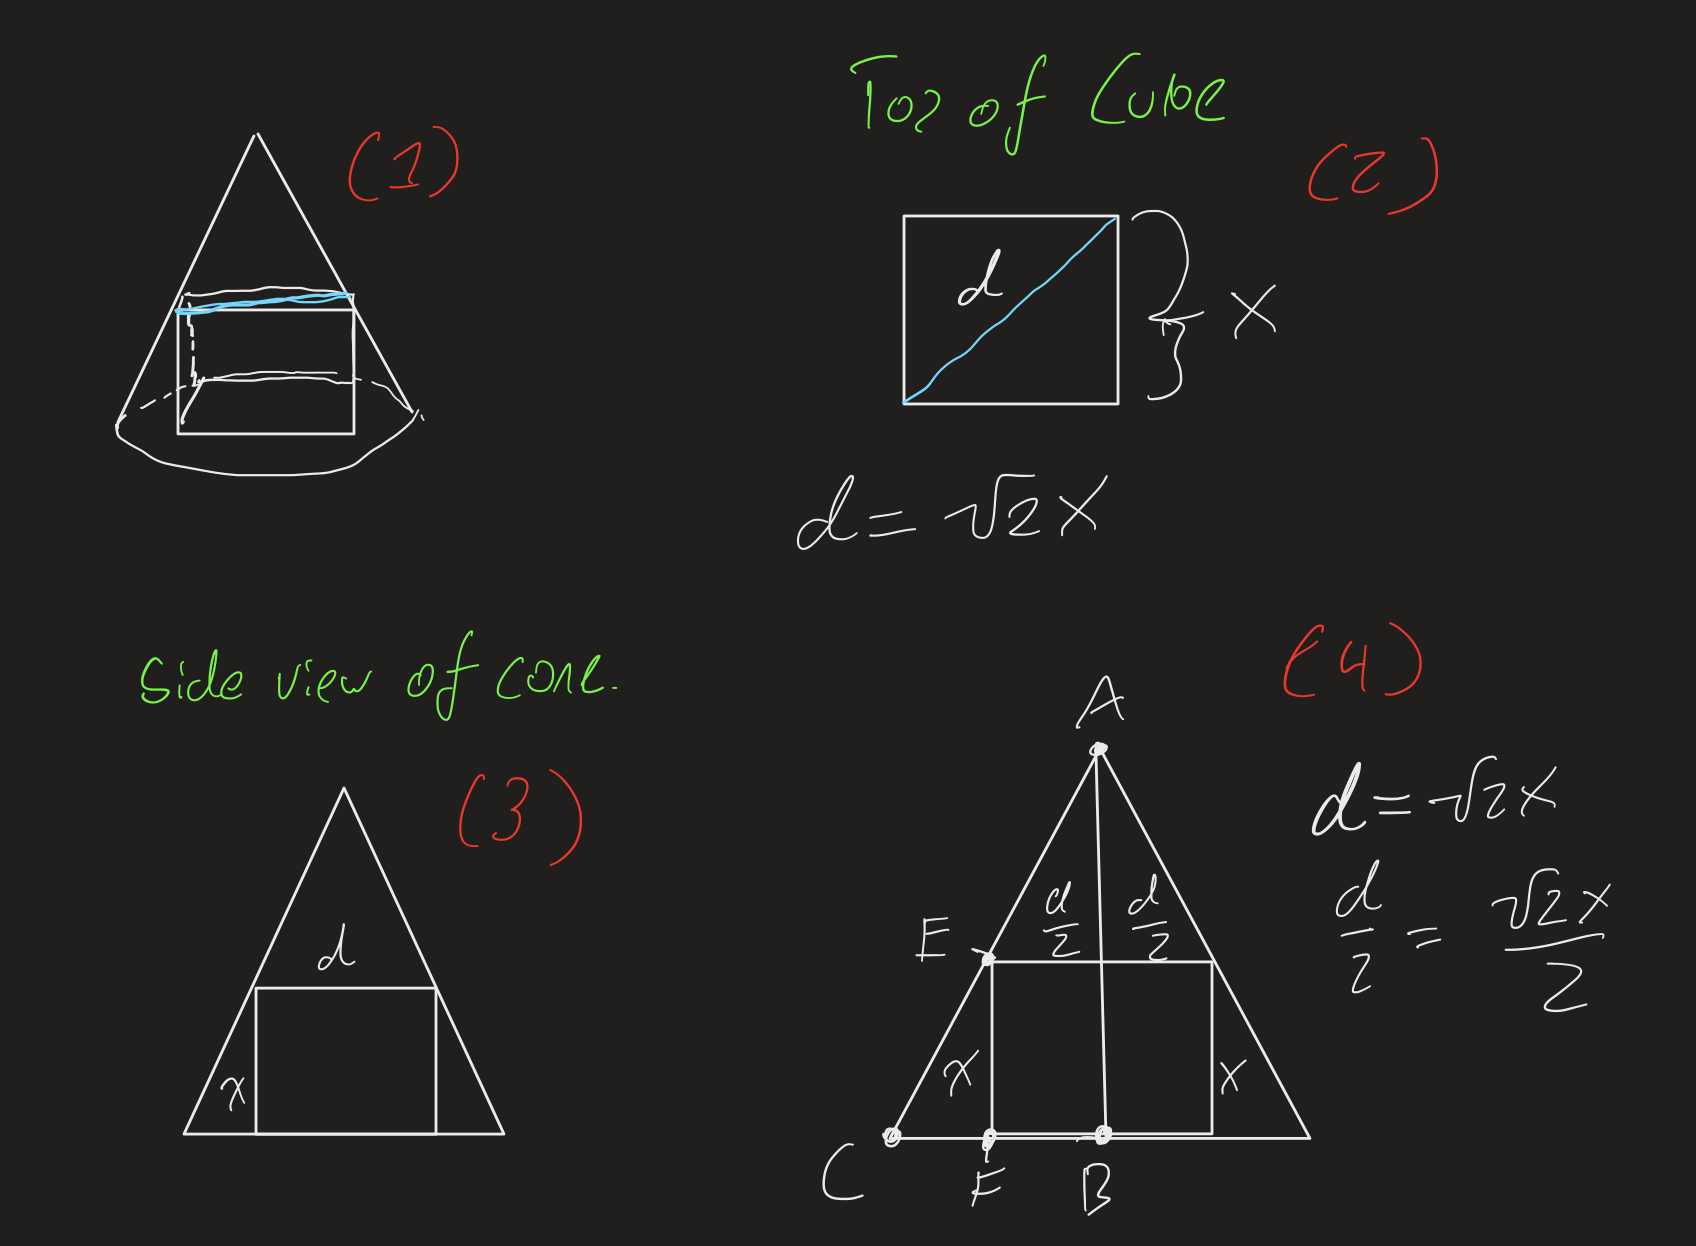
\includegraphics[scale=0.5]{diagram}
\begin{proof}
    Consider the cube inscribed in a cone as in image (1), where the lengths of each side are denoted by $x$, and the diagonal of the top of the cube is denoted by $d$ as seen in (2). We know that $d = \sqrt2 x$. Now consider the side view of the cone such that our view is perpendicular to the top diagonal of the square, giving us a triangle as seen in (3). We can bisect this triangle perpendicular to its base to obtain two more triangles as seen in (4). Each of these new triangles will then have a rectangle of side lengths $x$ and $\frac{d}{2}$ inside of them. We see that the triangle formed by $\triangle ABC$ is similar to $\triangle CEF$. This gives us the following equation,
    \begin{align*}
        \frac{1}{3} = \frac{1-\frac{d}{2}}{x} = \frac{1- \frac{\sqrt2 x}{2}}{x}
    \end{align*}
    now let's solve for $x$,
    \begin{align*}
        x &= 3 - \frac{3\sqrt2 x}{2}\\
        x + \frac{3\sqrt2 x}{2} &= 3 \\
        x(1 + \frac{3\sqrt 2}{2}) &= 3 \\
        x &= \frac{3}{1 + \frac{3\sqrt2}{2}} \approx 0.9661
    \end{align*}
\end{proof}

\begin{tcolorbox}
    \begin{problem} {IC | 12/03 | PP 41.}
        Find the minimum value of $\dfrac{(x+\frac{1}{x})^{6} - (x^{6}+\frac{1}{x^{6}}) -2)}{(x+\frac{1}{x})^{3} + (x^{3} + \frac{1}{x^{3}})}$ for $x > 0$
    \end{problem}
\end{tcolorbox}
\begin{proof}
    First let us manipulate the numerator of the given equation so that we can substitute $x + \frac{1}{x}$ with $y$.
    \begin{align*}
        (x+\frac{1}{x})^{6} - (x^{6} + \frac{1}{x^{6}}) -2 &= (x+ \frac{1}{x})^{6} - (x^{2} + \frac{1}{x^{2}})(x^{4} + \frac{1}{x^{4}} - 1) - 2 \\
        &= (x + \frac{1}{x})^{6} - ((x + \frac{1}{x})^{2}-2)((x^{2} + \frac{1}{x^{2}})^{2} - 3) - 2 \\
        &= (x + \frac{1}{x})^{6} - ((x + \frac{1}{z})^{2} - 2)(((x + \frac{1}{x})^{2} - 2)^{2} -3) - 2 \\
        &= y^{6} - (y^{2} - 2)((y^{2}-2)^{2} - 3) - 2 \\
        &= y^{6} - (y^{2} - 2)(y^{4}-4y^{2} + 1) -2 \\
        &= 4y^{2} - y^{2} + 2y^{4} -8y^{2} \\
        &= 6y^{4} - 9y^{2} && (1)
    \end{align*}
    Now let us do the same for the denominator of the given equation.
    \begin{align*}
        (x + \frac{1}{2})^{3} + (x + \frac{1}{x})(x^{2} + \frac{1}{x^{2}} -1) &= (x + \frac{1}{x'})^{3} + (x + \frac{1}{x})((x + \frac{1}{x})^{2} - 3) \\
        &= y^{3} + y(y^{2} - 3) \\
        &= 2y^{3} - 3y && (2)
    \end{align*}
    (1) and (2) together means,
    \begin{align*}
        \dfrac{(x+\frac{1}{x})^{6} - (x^{6}+\frac{1}{x^{6}}) -2)}{(x+\frac{1}{x})^{3} + (x^{3} + \frac{1}{x^{3}})} = \frac{6y^{4} - 9y^{2}}{2y^{3} - 3y} &= 3y \\ 
        &= 3(x + \frac{1}{x})
    \end{align*}
    We know though for $x > 0$ that $(x + \frac{1}{x})$ is bounded below by $2$, therefore,
    \begin{align*}
        3(x + \frac{1}{x}) \geq 3\cdot 2 = 6
    \end{align*}
    So $6$ is the minimum value of the given equation for $x> 0$
\end{proof}

\newpage
\begin{tcolorbox}
  \begin{problem} {IC | 12-03 | PP 42}
    Let $k > 1$ be a positive integer. Show that the equation $x^{2} -y^{2} = k^{3}$
always has integral solutions in $x$ and $y$.
  \end{problem}
\end{tcolorbox}
\begin{proof}
    Consider the following,
    \begin{align*}
        x^{2} - y^{2} &= k^{3} \\
        (x+y)(x-y) &= (k^{2})(k) && (1)
    \end{align*}
    (1) gives us the system of equations,
    \begin{align*}
        (x+y) &= k^{2} \\
        (x-y) &= k.
    \end{align*}
    We know that $k^{2} - k$ and $k^{2} +k $ will yield an even integer for any $k \in \zz$. This allows us to set $x = \frac{k^{2} + k}{2}$ and $y = \frac{k^{2} - k}{2}$. We see then,
    \begin{align*}
        (x+y)(x-y) &= (\frac{k^{2} + k}{2} + \frac{k^{2} - k}{2})(\frac{k^{2} + k}{2} -\frac{k^{2} - k}{2}) \\
        &= \frac{2k^{2}}{2}\frac{2k}{2} \\
        &= k^{2}k\\
        &= k^{3}
    \end{align*}
    meaning $x^{2}-y^{2} = k^{3}$ always has integral solutions in $x$ and $y$, by simply setting $x = \frac{k^{2} + k}{2}$ and $y = \frac{k^{2} - k}{2}$.
\end{proof}

\begin{tcolorbox}
    \begin{problem} {OC | 10/15 | 37 (Putnam)}
        Prove that there exist infinitely many integers $n$ such that $n,n+1,n +2$ are each the sum of the squares of two integers. 
    \end{problem}
\end{tcolorbox}
\begin{proof}
    Let $k \in \zz$, then let $n = (2k^{2} + 1)^{2} -1$. We see we can express $n$ as the sum of the squares of two integers through the following,
    \begin{align*}
       n =  (2k^{2}+1)^{2} -1 &= (2k^{2} + 1)(2k^{2} + 1) -1 \\
        &= 4k^{4} +2k^{2} + 2k^{2} + 1 -1 \\
        &= 4k^{4} + 4k^{2} \\
        &= (2k^{2})^{2} + (2k)^{2}
    \end{align*}

    For $n+1$,
    \begin{align*}
         n +1 = (2k^{2} + 1)^{2} -1 + 1 = (2k^{2} + 1)^{2} + 0^{2}
    \end{align*}
    
    For $n+2$, 
    \begin{align*}
        n +2 = (2k^{2} +1)^{2} -1 + 2 = (2k^{2} +1)^{2} + 1^{2}
    \end{align*}
    Since $k \in \zz$, that means there is indeed an infinite number of $n$ that satisfy the given statement.
\end{proof}
\newpage
\begin{tcolorbox}
    \begin{problem} {OC | 11/22 | PP 19}
        Find all ordered pairs $(a,b)$ of positive integers for which
        \[\frac{1}{a} + \frac{1}{b} = \frac{3}{2018}\]
    \end{problem}
\end{tcolorbox}
\begin{proof}
    Let us manipulate the given equation,
    \begin{align*}
         2018\frac{1}{a} + 2018\frac{1}{b} &= 3 \\
         2018b + 2018a &= 3ab \\
         0 &= 3ab -2018a -2018b \\
         0 &= 9ab - (3)2018a - (3)2018b \\
         2018^{2} &= 9ab -(3)2018a - (3)2018b + 2018^{2} \\
         2018^{2} &= (3a-2018)(3b - 2018) && (1)
    \end{align*}

    We know $2018^{2} \equiv 1 \text{ mod }3$ therefore each factor in (1) most be congruent to $1$ mod $3$. The set of factors of $2018^{2}$ that are congruent to $1$ mod $3$ are,
    \[\set{2^{2}1009^{2}, 1009^{2}, 2^{2}1009, 1009, 2^{2}, 1} = X.\]
    Therefore we can determine the values of $a$ and $b$ by simply solving for $(3a - 2018) = x $ for $x \in X$. Calculating this, it gives us the following possible pairs which will satisfy the given equation,
    \[(674, 340033),\ (673, 1358114),\ (1009,2018), \ (2018,1009), \ (1358114, 673), \ (340033, 674)\] 
\end{proof}

\begin{tcolorbox}
    \begin{problem} {OC | 11/22 | PP 20.}
        Let $S$ be the smallest set of positive integers such that,
        \begin{itemize}
            \item[(a)] 2 is in $S$.
            \item[(b)] $n$ is in $S$ whenever $n^2$ is in $S$
            \item[(c)] $(n+5)^{2}$ is in $S$ whenever $n$ is in $S$  
        \end{itemize}
        what positive integers are not in $S$?
    \end{problem}
\end{tcolorbox}
\begin{proof}
    Our claim is that,
    \begin{align*}
        S = \set{x \in \zz^{+} \mid x \neq 1,\ 5 \nmid x}
    \end{align*}
    in other words the integers $1$ and multiples of $5$ are not in $S$. First we will show that $S$ satisfies the 3 requirements. 

    For (a) it is obvious that $2 \neq 1$ and $5 \nmid 2$ therefore $S$ contains 2. 

    For (b) we know $5 \mid n^{2}$ if and only if $5 \mid n$. We also know $1^{2} = 1 \notin S$. Therefore for any $n^{2} \in S$ we have that $n \in S$.

    For (c) it follows simply from (b) since if $n \in S$ we have that $5\nmid n $ and therefore $5\nmid n+5$ which means $5 \nmid (n+5)^{2}$ thus $(n+5)^{2} \in S$.

    Now we just need to show that $S$ is indeed the smallest set of positive integers that satisfy these 3 requirements. We achieve this by showing if any other set, $S'$, satisfies these requirements then $S = S'$.

    Take $x \in S'$. Then by (c) $(x + 5)^{2} \in S'$ and by (b) we have $(n +5) \in S'$. We can note this consequence as, \[(*)\ \text{If }x \in S'  \rightarrow x+5k \in S', \ k \geq 0\] Now we know $2$ has to be in $S'$, which gives us the following implications,
    \begin{align}
        (2 + 5)^{2} = 49 &\in S' && \text{By (c)} \\
        (49 + 5)^{2} = (54)^{2} &\in S' && \text{By (c)} \\
        (54)^{2} + 5\cdot 44 = 56^{2} &\in S' && \text{By (*) where $k = 44$} \\
        56 &\in S' && \text{By (b)} \\
         56 + 5\cdot 13 = 121 &\in S' && \text{By (*) where $k = 13$} \\
         121 = 11^{2}, \ 11 &\in S' && \text{By (b)} \\
         11 + 5 = 16 &\in S' && \text{By (*) where $k = 1$} \\
         16 = 4^{2}&\in S' && \text{By (b)} \\
         4 + 5 = 9 &\in S' && \text{By (*)} \\
         9 = 3^{2} &\in S' && \text{By (b)}  
    \end{align}

    What we want to take away from these implications is that because $2$ is in $S'$ then so are $3,4$. Now let us resume from the fact that $16 \in S'$ which we know from line (7),
    \begin{align}
        16 + 5 \cdot 4 = 36 &\in S' && \text{By (*) where $k = 4$} \\
        36 = 6^{2}, \ 6 &\in S' && \text{By (b)}
    \end{align}

    Now we know that if a set $S'$ satisfies the 3 requirements then we know $2,3,4,6 \in S'$ then by applying $(*)$ to each of these values for all $k\geq 0$,
    \begin{align*}
        S' = \set{x \in \zz^{+}\mid x \neq 1, \ 5 \nmid x}
    \end{align*}
    which means $S = S'$, therefore $S$ is indeed the smallest set of positive integers satisfying these requirements.
\end{proof}

\end{document}